\section{Introduction}
Accurate sentence boundary detection (SBD) forms the foundation of natural language processing pipelines, \cite{gillick2009sentence, read2012sentence, schweter2019deep} including for large-scale legal applications such as M\&A due diligence, contract review, and legal research. While considered largely solved for general text, legal documents present unique challenges that cause standard approaches to fail in critical ways.

Legal text contains domain-specific patterns that confound general-purpose sentence boundary detectors: legal citations (e.g., \textit{United States v. Carroll Towing Co.}, 159 F.2d 169 (2d Cir. 1947)); specialized abbreviations (e.g., ``Corp.'', ``Inc.'', ``U.S.C.''); legal sources (e.g., ``Harv. L. Rev.''); numbered lists; and complex sentence structures. These features cause standard SBD tools to incorrectly split sentences or miss boundaries altogether, fundamentally compromising downstream legal analysis tasks.

Retrieval-augmented generation (RAG) systems are increasingly used in the legal domain. \cite{pipitone2024legalbench, wiratunga2024cbr, hindi2025enhancing}  False positives are especially detrimental in such RAG style systems, as they fragment logically connected legal concepts across multiple chunks, leading to reasoning failures. As illustrated in Figure \ref{fig:rag-error-cascade}, the relationship between precision and fragmentation follows an inverse exponential curve, where each percentage point improvement in precision yields progressively greater reductions in fragmentation errors. This non-linear effect occurs because each correctly preserved sentence boundary prevents multiple downstream failures throughout the RAG pipeline. High-throughput processing is equally crucial for legal applications involving millions of documents.

\begin{figure*}[t]
\centering
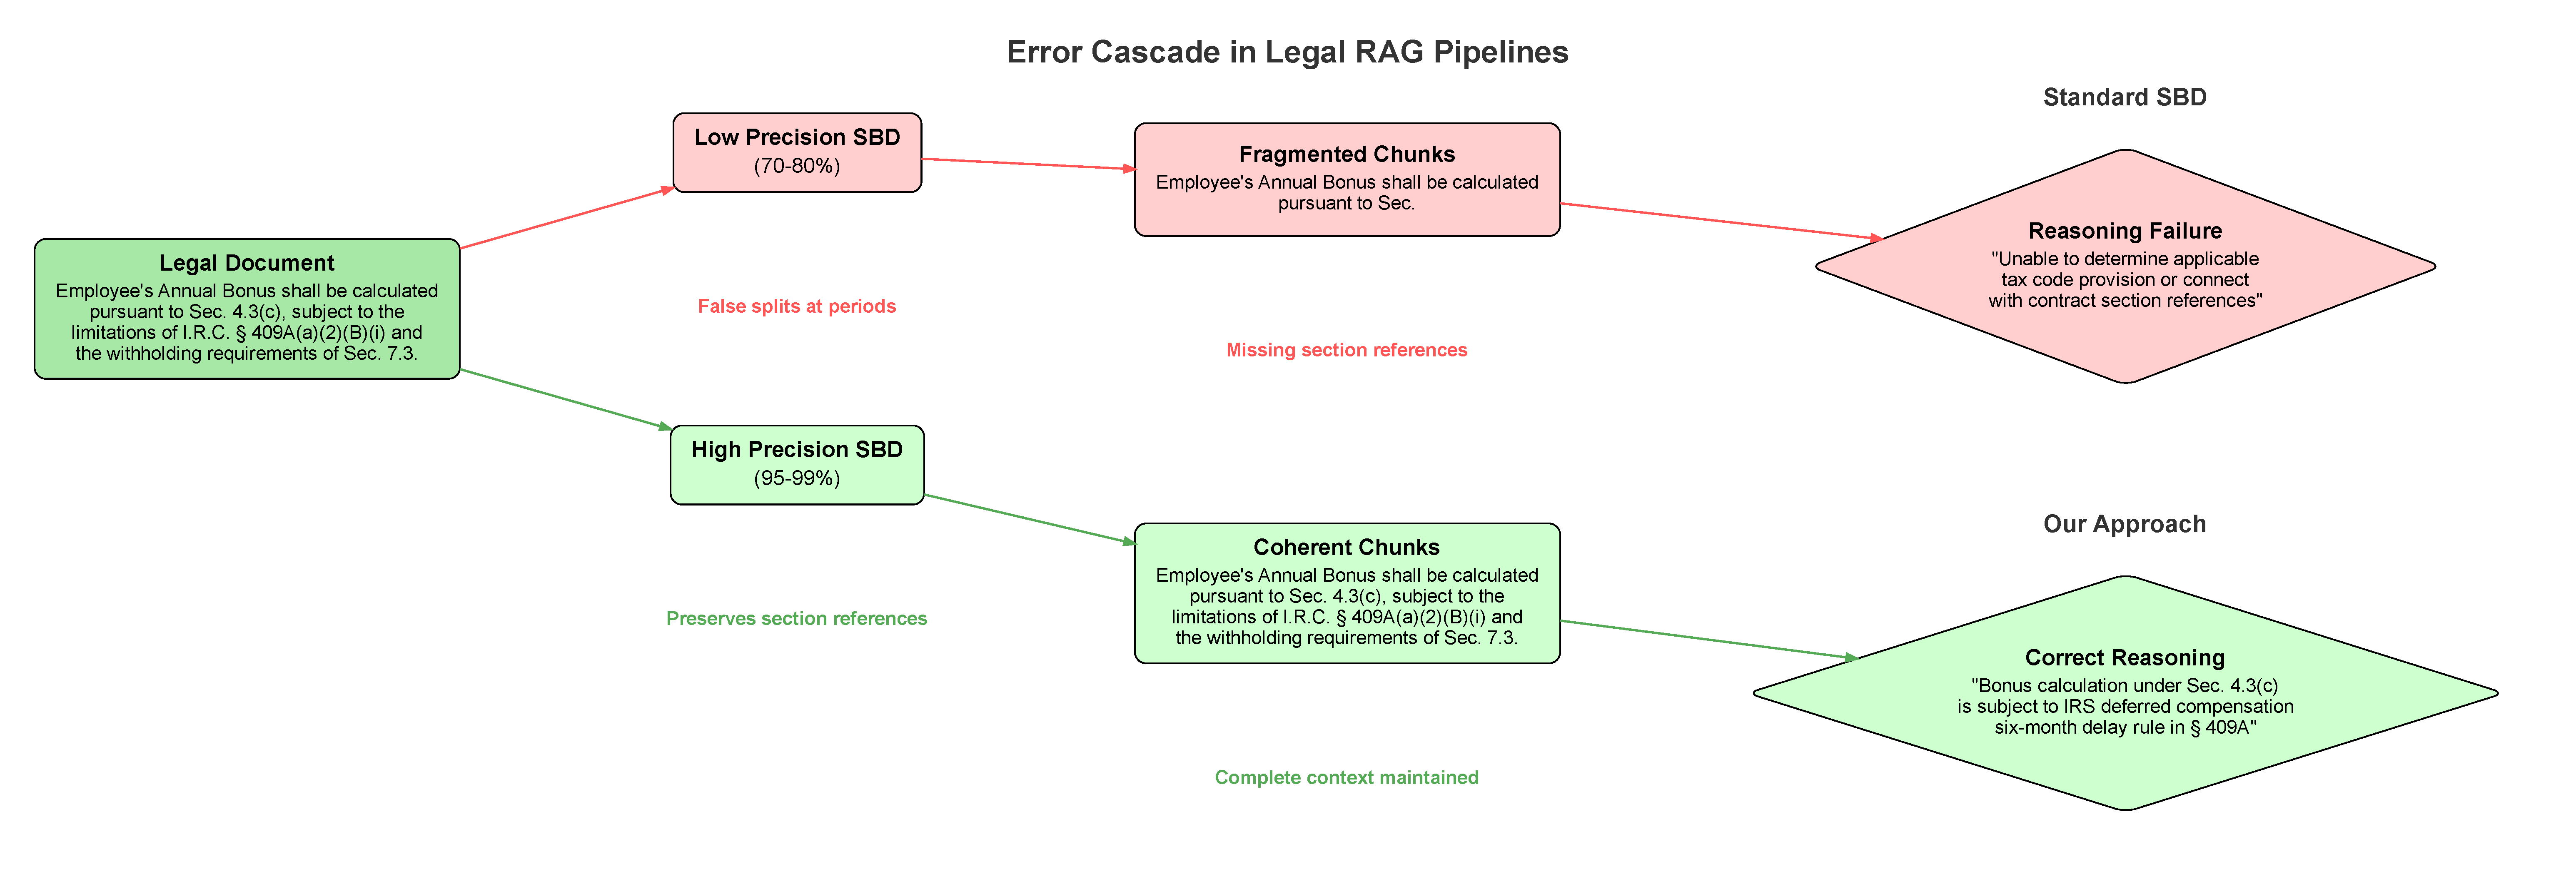
\includegraphics[width=1.05\textwidth]{figures/rag_error_cascade.pdf}
\caption{Error cascade in legal RAG pipelines from low-precision SBD to downstream reasoning failures.}
\label{fig:rag-error-cascade}
\end{figure*}

For example, when processing \textit{``Employee's Annual Bonus shall be calculated pursuant to Sec. 4.3(c), subject to the limitations of I.R.C. § 409A(a)(2)(B)(i) and the withholding requirements of Sec. 7.3,''} a standard SBD system incorrectly splits after ``Sec. 4.3'', creating multiple fragments. When queried about bonus calculation rules, a RAG system would retrieve only partial information, missing critical context about the IRC §409A tax code limitations that affect deferred compensation.

In this paper, we introduce two new open-source SBD libraries optimized for high-precision, high-throughput processing of legal text:
\\
\begin{itemize}
    \item \textbf{NUPunkt}: A pure Python implementation that extends the unsupervised Punkt algorithm by Kiss and Strunk \cite{kiss2006unsupervised} with legal domain optimizations and training on the significantly larger KL3M legal corpus \cite{kl3m-data}. NUPunkt achieves 91.1\% precision while processing 10 million characters per second with modest memory requirements (432 MB), providing a 29-32\% precision improvement over standard tools like NLTK Punkt (62.1\%) and spaCy (64.3-64.7\%), with zero external dependencies and MIT licensing.
    \\
    \item \textbf{CharBoundary}: A family of character-level machine learning models, inspired by character-based approaches like Sanchez \cite{sanchez2019sentence} but trained on substantially more diverse legal text, in three sizes (small, medium, large) that offer balanced precision-recall tradeoffs. The large model achieves the highest F1 score (0.782) among all tested methods, with throughput ranging from 518K-748K characters per second depending on model size. CharBoundary requires only scikit-learn and optional ONNX runtime integration, and is also available under the MIT license.
    \\
\end{itemize}

Our experimental evaluation on five diverse legal datasets comprising over 25,000 documents and 197,000 annotated sentence boundaries demonstrates that both libraries significantly outperform general-purpose alternatives. NUPunkt excels in precision-critical applications where minimizing false positives is paramount, enabling processing of multi-million document collections in minutes rather than hours. CharBoundary models provide the best overall F1 scores with excellent balance between precision and recall, making them suitable for applications requiring more nuanced boundary detection.

Our contributions include: (1) two open-source SBD libraries optimized for legal text with specific focus on precision and throughput; (2) a comprehensive benchmark of sentence boundary detection performance across diverse legal datasets; and (3) detailed analysis of precision-throughput tradeoffs for legal text processing applications. Both libraries are freely available under the MIT license, with interactive demonstrations at \url{https://sentences.aleainstitute.ai/}. All source code to replicate this paper's experiments will be available at \url{https://github.com/alea-institute/legal-sentence-paper}.